Finally, we're closing in on Smirnov's approach to the~$abc$-conjecture via geometry over the field with one element.

\subsection{The geometric defect}

Let~$\phi\colon C_1 \mapsto C_2$ be a cover of curves defined over~$k$, then the scheme-version of the Riemann-Hurwitz inequality is
\begin{equation}
  2 \genus_{C_1} - 2 \geq \deg(\phi) (2 \genus_{C_1} -2) + \sum^{\text{scheme}}_{P \in C_1} (e_{\phi}(P)-1) \deg(P)
\end{equation}

In the special case, when~$f$ is a non-constant rational function in~$k(C)$ and the corresponding cover is~$f\colon C \mapsto \mathbb{P}^1_k$, this reads
\begin{equation}
  2\genus_C-2 \geq -2 \deg(f) + \sum^{\text{scheme}}_{P \in C} (e_f(P)-1) \deg(P)
\end{equation}
which can be turned into the inequality
\begin{equation}
  \sum^{\text{scheme}}_{P \in C} \frac{(e_f(P)-1) \deg(P)}{\deg(f)} \leq 2 - \frac{2-2\genus_C}{\deg(f)}
\end{equation}

We call the expression
\begin{equation}
  \delta(P) \coloneqq \tfrac{(e_f(P)-1) \deg(P)}{\deg(f)}  
\end{equation}
the \emph{defect} of~$P$. Observe that~$\delta(P) \geq 0$ and so this inequality only improves it we restrict the summation to some subset of schematic~$C$-points.

\subsection{The arithmetic defect}

Take a positive rational number~$q = \frac{m}{n}$ with~$1 \leq n < m$ and~$(m,n)=1$ and consider the cover
\begin{equation}
  q\colon\Spec(\mathbb{Z}) \mapsto \mathbb{P}^1 / \mathbb{F}_1.
\end{equation}

Recall that the fiber over the point~$[d] \in \mathbb{P}^1 / \mathbb{F}_1$ consists of all prime divisors of~$m^d-n^d$ not dividing any~$m^e-n^e$ for~$e < d$. The fiber of~$[0]$ (resp. of~$[\infty]$) consists of all prime divisors of~$m$ (resp. of~$n$ together with~$\infty$). Here's part of the cover for~$q=\frac{104348}{33215}$ (a \href{http://mathworld.wolfram.com/PiApproximations.html}{good rational approximation} for~$\pi$).

\begin{figure}[ht]
  \centering
  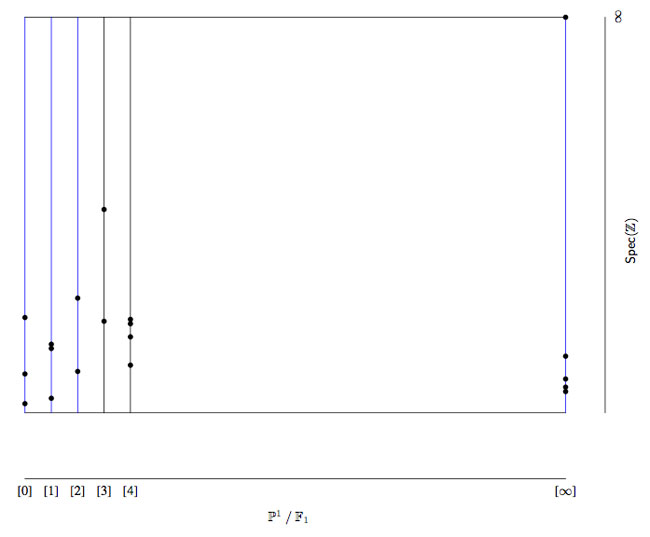
\includegraphics[width=11cm]{f1-abc/pimap.jpg}
  \caption{Impression of the cover~$q=104348/33215$}
  \label{figure:pi-map}
\end{figure}

It is tempting to define the ramification index~$e_q(p)$ for the map~$q$ in the prime~$p$ lying in the fiber~$q^{-1}([d])$ to be the largest power of~$p$ dividing~$m^d-n^d$. Likewise, for~$p \in q^{-1}([0])$ (resp.\ in~$q^{-1}([\infty])$) take for~$e_q(p)$ the largest power of~$p$ dividing~$m$ (resp. dividing~$n$). Finally, take~$e_q(\infty) = \log(q)$.

Combine this with our previous definitions for the degree of~$p$ to be~$\log(p)$ and of the degree of the map~$q$ to be~$\log(m)$, to define the arithmetic defect of~$q$ in the prime~$p$ to be
\begin{equation}
  \delta(p) = \frac{(e_q(p)-1) \log(p)}{\log(m)}
\end{equation}
We can now define the total defect of the cover~$q$ over the point~$[d] \in \mathbb{P}^1 / \mathbb{F}_1$ to be
\begin{equation}
  \delta_{[d]} = \sum_{\mathclap{p \in q^{-1}([d])}} \delta(p).
\end{equation}

It is easy to work out these total defects for the four~$\mathbb{F}_1$-rational points of~$\mathbb{P}^1 / \mathbb{F}_1$:\ $\{ [0],[1],[2],[\infty] \}$ (the primes lying on the blue lines in the graph). 

For a natural number~$a$ let~$a_0$ be its square-free part and~$a_1 = \tfrac{a}{a_0}$ the remaining part. Then
\begin{equation}
  \left\{
  \begin{aligned}
	  \delta_{[0]} &= \frac{\log(m_1)}{\log(m)} \\
	  \delta_{[\infty]} &= \frac{\log(n_1)+\log(q)-1}{\log(m)} \\
	  \delta_{[1]} &= \frac{\log((m-n)_1)}{\log(m)} \\
	  \delta_{[2]} &= \frac{\log(k_1)}{\log(m)}
  \end{aligned}
  \right.
\end{equation}
where~$k$ is~$m+n$ divided by the largest~$2$-power it may contain. 

\subsection{Hurwitz-conjecture for~$\mathbb{Q}$}

If we sum the defects of~$q$ in all primes over the points~$\{ [0],[1],[\infty] \}$ we would get, in analogy with the Hurwitz-inequality in the function field case
\begin{equation}
  \delta_{[0]}+\delta_{[1]}+\delta_{[\infty]} \leq 2 - \frac{2 - 2\genus_{\Spec(\mathbb{Z})}}{\log(m)}
\end{equation}

We do not know what the genus of the arithmetic curve~$\Spec(\mathbb{Z})$ might be, but is sure is a constant not depending on the map~$q$. If we could develop a geometry over~$\mathbb{F}_1$ such that all wild guesses we made before would turn out to be the correct ones for an~$\mathbb{F}_1$-version of the Hurwitz inequality, we would have the statement below:

For every~$\epsilon > 0$ there exists a constant~$C_\epsilon$ such that the following inequality holds for every pair~$1 \leq m < n$ with~$(m,n)=1$
\begin{equation}
  \frac{\log(m_1) + \log((m-n)_1) + \log(n_1) + \log(m)-\log(n)-1}{\log(m)} \leq 2 + \epsilon + \frac{C_\epsilon}{\log(m)}.
\end{equation}

\subsection{The ``proof'' of the~$abc$-conjecture}

The~$abc$-conjecture requires for every~$\epsilon > 0$ a constant~$D_\epsilon$ such that for all coprime natural numbers~$a$ and~$a$ we have with~$a+b=c$
\begin{equation}
c \leq D_\epsilon a_0b_0c_0)^{1+\epsilon}
\end{equation}

Well, take~$m=c$ and~$n=\min(a,b)$ then in the conjectural Hurwitz inequality for the cover corresponding to~$q=\frac{m}{n}$ above we have that
\begin{equation}
  \begin{aligned}
    \frac{\log(m_1)}{\log(m)} &= 1 - \frac{\log(m_0)}{\log(m)} \\
    \frac{\log(n_1)+\log(m)-\log(n)-1}{\log(m)} &= 1 - \frac{\log(n_0)}{\log(m)} - \frac{1}{\log(m)} \\
    \frac{\log((m-n)_1)}{\log(m)}&=\frac{\log(m-n)}{\log(m)}-\frac{\log((m-n)_0)}{\log(m)} \\
    &\geq 1 - \frac{\log((m-n)_0)}{\log(m)} - \frac{\log(2)}{\log(m)}
  \end{aligned}
\end{equation}
(the latter inequality because~$m-n \geq \frac{m}{2}$ and so~$\log(m-n) \geq \log(m)-\log(2)$). Plug this into the inequality above and get
\begin{equation}
  3-\frac{\log(n_0m_0(m-n)_0)}{\log(m)} \leq 2 + \epsilon + \frac{c(\epsilon) + 1 + \log(2)}{\log(m)}
\end{equation}

Take~$\log(c'(\epsilon))=c(\epsilon)+1+\log(2)$ and reshuffle in order to get the inequality~$m^{1-\epsilon} \leq c'(\epsilon)(n_0m_0(m-n)_0)$. But then, finally (finally!) with~$D_\epsilon=c'(\epsilon)^{1+\epsilon}$
\begin{equation}
  c=m \leq D_\epsilon(n_0m_0(m-n)_0)^{1+\epsilon} = D_\epsilon(a_ob_0c_0)^{1+\epsilon}.
\end{equation}
